% Schematic of the actual response comparison, not measured vectors.
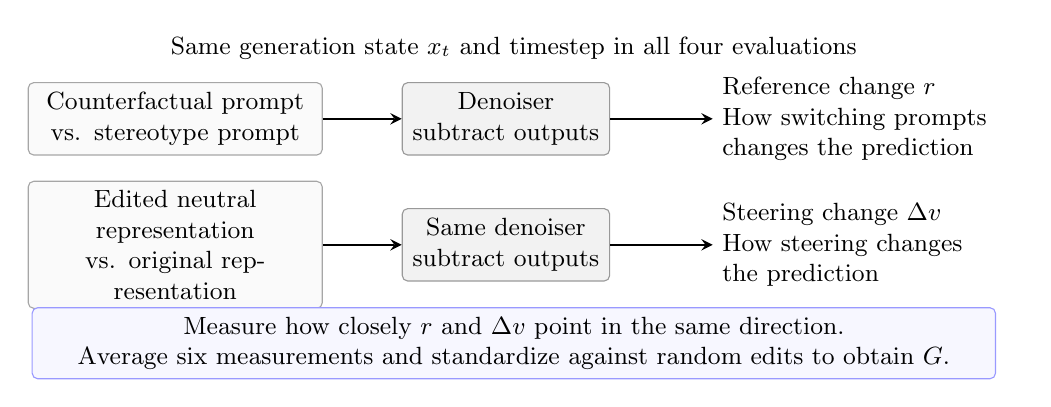
\begin{tikzpicture}[x=1cm,y=1cm,>=stealth,
  cond/.style={draw=black!35,rounded corners=2pt,fill=black!2,align=center,text width=3.5cm,minimum height=.92cm,font=\small},
  model/.style={draw=black!40,rounded corners=2pt,fill=black!5,align=center,text width=2.4cm,minimum height=.92cm,font=\small},
  resp/.style={align=left,text width=3.7cm,font=\small}]
\node[font=\small] at (6.1,2.55) {Same generation state $x_t$ and timestep in all four evaluations};
\node[cond] (pair) at (1.8,1.65) {Counterfactual prompt\\vs. stereotype prompt};
\node[model] (den1) at (6.0,1.65) {Denoiser\\subtract outputs};
\node[resp] (ref) at (10.6,1.65) {Reference change $r$\\How switching prompts\\changes the prediction};
\draw[->,thick] (pair)--(den1);\draw[->,thick] (den1)--(ref);
\node[cond] (write) at (1.8,.05) {Edited neutral representation\\vs. original representation};
\node[model] (den2) at (6.0,.05) {Same denoiser\\subtract outputs};
\node[resp] (delta) at (10.6,.05) {Steering change $\Delta v$\\How steering changes\\the prediction};
\draw[->,thick] (write)--(den2);\draw[->,thick] (den2)--(delta);
\node[draw=blue!40,fill=blue!3,rounded corners=2pt,align=center,text width=12cm,minimum height=.75cm,font=\small] at (6.1,-1.2)
{Measure how closely $r$ and $\Delta v$ point in the same direction.\\Average six measurements and standardize against random edits to obtain $G$.};
\end{tikzpicture}
